\documentclass{beamerthemeMono}

% specify some optional logos
\graphicspath{{figures/}}
%\pgfdeclareimage[height=1.45cm]{mainlogo}{figures/logo}
\pgfdeclareimage[height=1.4cm]{mainlogo}{figures/logo.pdf}
% placed in the lower left/right corner if the \pgfuseimage{minilogo}
% command is uncommented in the \institute command below.
\pgfdeclareimage[height=1cm]{minilogo}{figures/logo.pdf}
\logo{\pgfuseimage{minilogo}}

\AtBeginSection[] {
  \begin{frame}
    \frametitle{目录} 
    {\tableofcontents[%
      currentsection, % causes all sections but the current to be shown in a semi-transparent way.
%     currentsubsection, % causes all subsections but the current subsection in the current section to ...
      hideallsubsections, % causes all subsections to be hidden.
%     hideothersubsections, % causes the subsections of sections other than the current one to be hidden.
%      part=2 % part number causes the table of contents of part part number to be shown
%     pausesections, % causes a \pause command to be issued before each section. This is useful if you
%     pausesubsections, %  causes a \pause command to be issued before each subsection.
      %sections={<1-3|handout:0>} %{ overlay specification },
      ]}
   \end{frame}}

\makeatletter
\AtBeginPart{%
  \beamer@tocsectionnumber=0\relax
  \setcounter{section}{0}
  \frame[plain]{\partpage}%
}
\makeatother

% \AtBeginPart{
%      \begin{frame}[plain]
%          \partpage
%      \end{frame}}

% \AtBeginSubsection[]                            % 在每个子段落之前
% {
%   \frame{                                         % handout:0 表示只在手稿中出现
%     \frametitle{目录} \small
%     \tableofcontents[
%       currentsection,
%       currentsubsection,
%       subsectionstyle=show/shaded/hide]
%   }
% }
%%%%%%%%%%%%%%%%%%%%%%%%%%%%%%%%%%%%%%%%%%%%%%%%%%%%%%%%%%%%
%%%%%%%%%%%%%%%%%%%%%%%%%%%%%%%%%%%%%%%%%%%%%%%%%%%%%%%%%%%%
          % 文档开始
%%%%%%%%%%%%%%%%%%%%%%%%%%%%%%%%%%%%%%%%%%%%%%%%%%%%%%%%%%%%
%%%%%%%%%%%%%%%%%%%%%%%%%%%%%%%%%%%%%%%%%%%%%%%%%%%%%%%%%%%%

\begin{document}

\title[交通规划行业中的数据应用现状及思考]% optional, use only with long paper titles
{\heiti \xiaoerhao 交通规划行业中的数据应用现状及思考}


\author[邹海翔] % optional, use only with lots of authors
{\xiaosihao 邹海翔}
\date{\xiaosihao 2019年2月}
 % - Give the names in the same order as they appear in the paper.  -
 % Use the \inst{?} command only if the authors have different
 % affiliation. See the beamer manual for an example


\institute[综合交通所] % optional - is placed in the bottom of the sidebar on every slide
{%
   \xiaosihao 综合交通所
   % there must be an empty line above this line - otherwise some
   % unwanted space is added
   % between the university and the country (I do not know why)
}

 % \date{\today}
\titlegraphic{\pgfuseimage{mainlogo}} %insert a company or department logo


 % the titlepage the plain option removes the sidebar and header from
 % the title page
\begin{frame}[plain]
  \titlepage
\end{frame}
%%%%%%%%%%%%%%%%


\begin{frame}{目录}{}
   {\tableofcontents[hideallsubsections]}
\end{frame}

%%%%%%%%%%%%%%%%%%%%%%%%%%%%%%%%%%%%%%%%%%%%%%%%%%%%%%%%%%%%

%%%%%%%%%%%%%%%%%%%%%%%%%%%%%%%%%%%%%%%%%%%%%%%%%%%%%%%%%%%%
\section{大数据时代下的交通规划}
\subsection{交通规划业务}
\begin{frame}[t]{\subsecname}
\begin{itemize}
\item 交通规划是城市规划的重要组成部分,主要目的是\emphText{建设和改善城市交通系统},从城市规模、用地布局、道路组织等
源头出发,提出解决城市交通问题的对策和具体方案
\item 交通规划是一项\emphText{综合性业务},除了交通以外,还涉及城市空间、人口、土地利用、公共政策等多方面的因素
\item 交通规划的成果主要是\emphText{各层次的规划编制方案},用于辅助城市管理者的决策,并指导落实最终的建设实施
\end{itemize}

\begin{columns}
  \begin{column}{.4\textwidth}
    \begin{figure}\flushright
      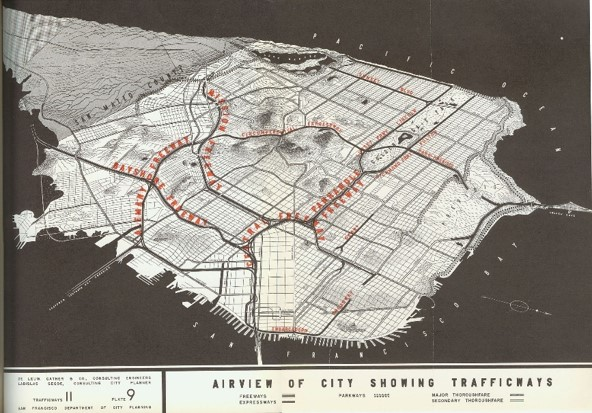
\includegraphics[height=0.3\textheight]{chp01_旧金山.jpg}
      \caption{1948年旧金山路网规划图}
    \end{figure}
  \end{column}
  \begin{column}{.6\textwidth}
    \begin{figure}\flushleft
      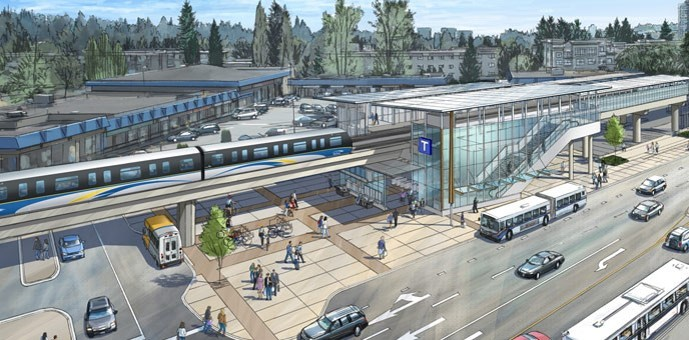
\includegraphics[height=0.3\textheight]{chp01_交通设计.jpg}
      \caption{城市公交站点交通设计图}
    \end{figure}
  \end{column}
\end{columns}
\end{frame}

\begin{frame}[t]{\subsecname}
\begin{itemize}
\item \emphText{交通调查}是交通规划业务最主要的数据来源,并以此为依据建立分析模型推断规划方案
\item 国内一般\emphText{5--10年}进行一次城市居民出行调查,每次调查的时间长达数月甚至一年
\end{itemize}

\begin{figure}
  \centering
  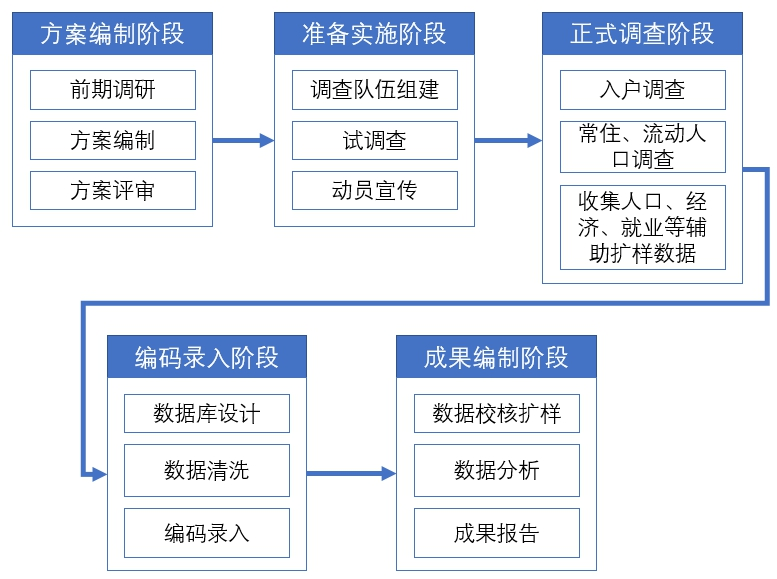
\includegraphics[width=0.65\textwidth]{chp01_交通调查.jpg}
  \caption{交通调查的一般流程}
\end{figure}
\end{frame}

\subsection{大数据业务}
\begin{frame}[t]{\subsecname}

\end{frame}

%%%%%%%%%%%%%%%%%%%%%%%%%%%%%%%%%%%%%%%%%%%%%%%%%%%%%%%%%%%%

%%%%%%%%%%%%%%%%%%%%%%%%%%%%%%%%%%%%%%%%%%%%%%%%%%%%%%%%%%%%
\section{交通规划中的数据}

%%%%%%%%%%%%%%%%%%%%%%%%%%%%%%%%%%%%%%%%%%%%%%%%%%%%%%%%%%%%

%%%%%%%%%%%%%%%%%%%%%%%%%%%%%%%%%%%%%%%%%%%%%%%%%%%%%%%%%%%%
\section{数据分析的``七种武器''}

%%%%%%%%%%%%%%%%%%%%%%%%%%%%%%%%%%%%%%%%%%%%%%%%%%%%%%%%%%%%

%%%%%%%%%%%%%%%%%%%%%%%%%%%%%%%%%%%%%%%%%%%%%%%%%%%%%%%%%%%%
\section{数据在业务中的应用案例}

%%%%%%%%%%%%%%%%%%%%%%%%%%%%%%%%%%%%%%%%%%%%%%%%%%%%%%%%%%%%

%%%%%%%%%%%%%%%%%%%%%%%%%%%%%%%%%%%%%%%%%%%%%%%%%%%%%%%%%%%%
\section{再认识与展望}

%%%%%%%%%%%%%%%%%%%%%%%%%%%%%%%%%%%%%%%%%%%%%%%%%%%%%%%%%%%%

%%%%%%%%%%%%%%%%%%%%%%%%%%%%%%%%%%%%%%%%%%%%%%%%%%%%%%%%%%%%

%%%%%%%%%%%%%%%%%%%%%%%%%%%%%%%%%%%%%%%%%%%%%%%%%%%%%%%%%%%%%%%%%%%%%%%%%%%%
% 结束页
%%%%%%%%%%%%%%%%%%%%%%%%%%%%%%%%%%%%%%%%%%%%%%%%%%%%%%%%%%%%%%%%%%%%%%%%%%%%
\begin{frame}[plain,noframenumbering]%
  \finalpage{
    \begin{table} \Huge \centering
      \begin{tabular}{c}
        汇~报~结~束\\
        谢~谢!
      \end{tabular} \end{table}
    \titlegraphic{\pgfuseimage{mainlogo}}}
\end{frame}
\end{document}
%%% Local Variables:
%%% mode: latex
%%% TeX-master: t
%%% End:
